%!TEX root = ../document.tex
\chapter{Empirical settings and method}
The application is divided into three logical units: data collection, data processing and database, and user interface. In the following sections these units will be explained further. 

\begin{figure}
\centering
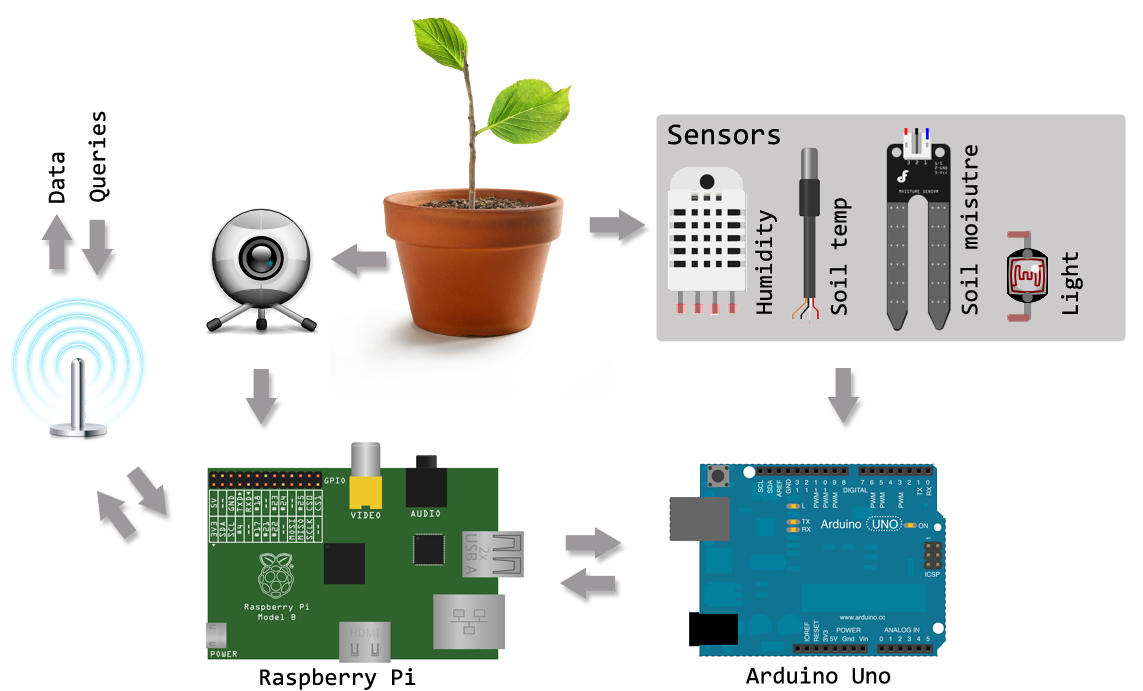
\includegraphics[width=1\textwidth]{img/hardware/application.png}
\caption{High-level illustration of the physical hardware components in the application}
\label{fig:application}
\end{figure}

\section{Plant data collection}
At the lowest level in the information hierarchy is the hardware and software responsible for capturing and uploading environmental data regarding the plant. Like a patient in a hospital, the plant is connected to a range of sensors, each responsible for reading a specific variable which is important for the plant’s functioning. These variables are then sent to a computer, processed, and uploaded to the next level in the data hierarchy. In the following sections we will follow the data on it’s way from the plant’s physical location to the cloud.

\subsection{Sensors}

\def\arraystretch{1.8}
\begin{table}
    \begin{tabular}{|l|p{250pt}|}
    \hline
    \textbf{Sensor}               & \textbf{Description}                                                                                                  \\ \hline
    TSL2561              & Digital luminosity sensor. Measures light in lux from 300-1100nm.                                            \\ \hline
    RHT03                & Digital humidity and temperature sensor. Measures relative humidity and temperature in celsius.              \\ \hline
    DS18B20              & Digital waterproof temperature sensor. Measures temperature in celsius                                       \\ \hline
    DFRobot sku:sen0114  & Analog soil moisture sensor. Returns values between 0 and 900 depending on electrical conductivity of soil.  \\ \hline
    \end{tabular}
    \caption{Sensors used in the application}
\end{table}


With the advent of the \emph{“internet of things”}, sensors are becoming available in many different forms and packages. Just as LEGO-pieces they can be used in a wide range of applications. From automating tasks such as keeping a steady indoor-temperature, to measuring variables which we as humans cannot see. 

For this application we did a short review of the available off-the-shelf packages available on the market. 

The sensors are able to capture information about the environment and transform it to data variables which we can store and categorize. In total there are five different sensors connected to the plant, or in the plant’s vicinity: soil moisture, soil temperature, air temperature, humidity, and light. 


(write something about the sensortag)

The sensors we have used in this project works at the most basic level in the same way as a volume controller on an amplifier. On an amplifier one can adjust the volume by varying the resistance in the signal going to the speakers. If we turn the volume up, the resistance goes down, and if we turn the volume down, the resistance goes up. The concept with sensors is the same, only that instead controlling resistance with a volume knob, it is controlled by light, moisture or other environmental variables. 

The resistors used in the temperature sensors are called “thermistors”, and the way they operate is by varying the resistance according to the temperature. Since we already know how many volts we are sending to the thermistor on the one end, we can use the amount of volts we get back to calculate the resistance. In our application this is done by a voltage divider which uses a formula as follows: 

\begin{equation}
U_{out}=\frac{R_{2}}{R_{1}+R_{2}}\cdot U_{in} 
\label{eq:vdiv1}
\end{equation}
Where $V_{out}$ is voltage out, $U_{in}$ is voltage in, $R_{1}$ is a given resistance, and $R_{2}$ is the resistance we want to calculate. For this example let's assume that $U_{in} = 5_{v}$, $U_{out} = 2_{v}$, and $R_{1} = 1K\Omega$. We solve this equation with regard to $R_{2}$
\begin{equation}
R_{2} = \frac{U_{out} \cdot R_{1}}{U_{in}-U_{out}}
\end{equation} 

\begin{equation}
R_{2} = \frac{2V \cdot 1000\Omega}{5V-2V}
\end{equation} 

\begin{equation}
R_{2} = \frac{2000\Omega}{3}
\end{equation} 

\begin{equation}
R_{2} = 667\Omega
\end{equation} 

Then we can see that the calculated resistance is 667$\Omega$. This value can then be mapped to the correct unit of measure, in this case Celsius or Fahrenheit. 

As we are using digital sensors, all of these calculations are done internally in the sensors, and coded into a digital signal. This signal, consisting of 1s and 0s, is then passed onto the next unit in our system, the Arduino.  

\subsection{Arduino}
(Write about embedded systems. What other alternatives are there to the Arduino? )

Arduino is an open-source prototyping platform which makes it easy to interface low-level electronics (e.g sensors) with higher-level electronics (e.g computers). The core part of the Arduino is an Atmel\texttrademark Atmega microcontroller which can be programmed by a computer over usb, using the Arduino programming language and the Arduino development environment \citep{arduino}.

We have used an Arduino Uno which has 13 digital input output pins (GPIO), five analog inputs, i2c inputs, and USB for serial communication. The DSB18B20 soil temperature sensor and RHT03 temperature and humidity sensor are connected to the digital inputs through a 1K(ohm) pullup resistor. The pullup resistors are used to keep the voltage sent to the arduino from fluctuating when the sensor is not sending any data. The TSL2561 luminosity sensor is connected to the A4/SDA and A5/SDL ports of the Arduino as it communicates over the i2c protocol. And the DFRobot soil moisture sensor is connected to A3 (Analog input 3) as it outputs analog voltage.  

\begin{figure}
\centering
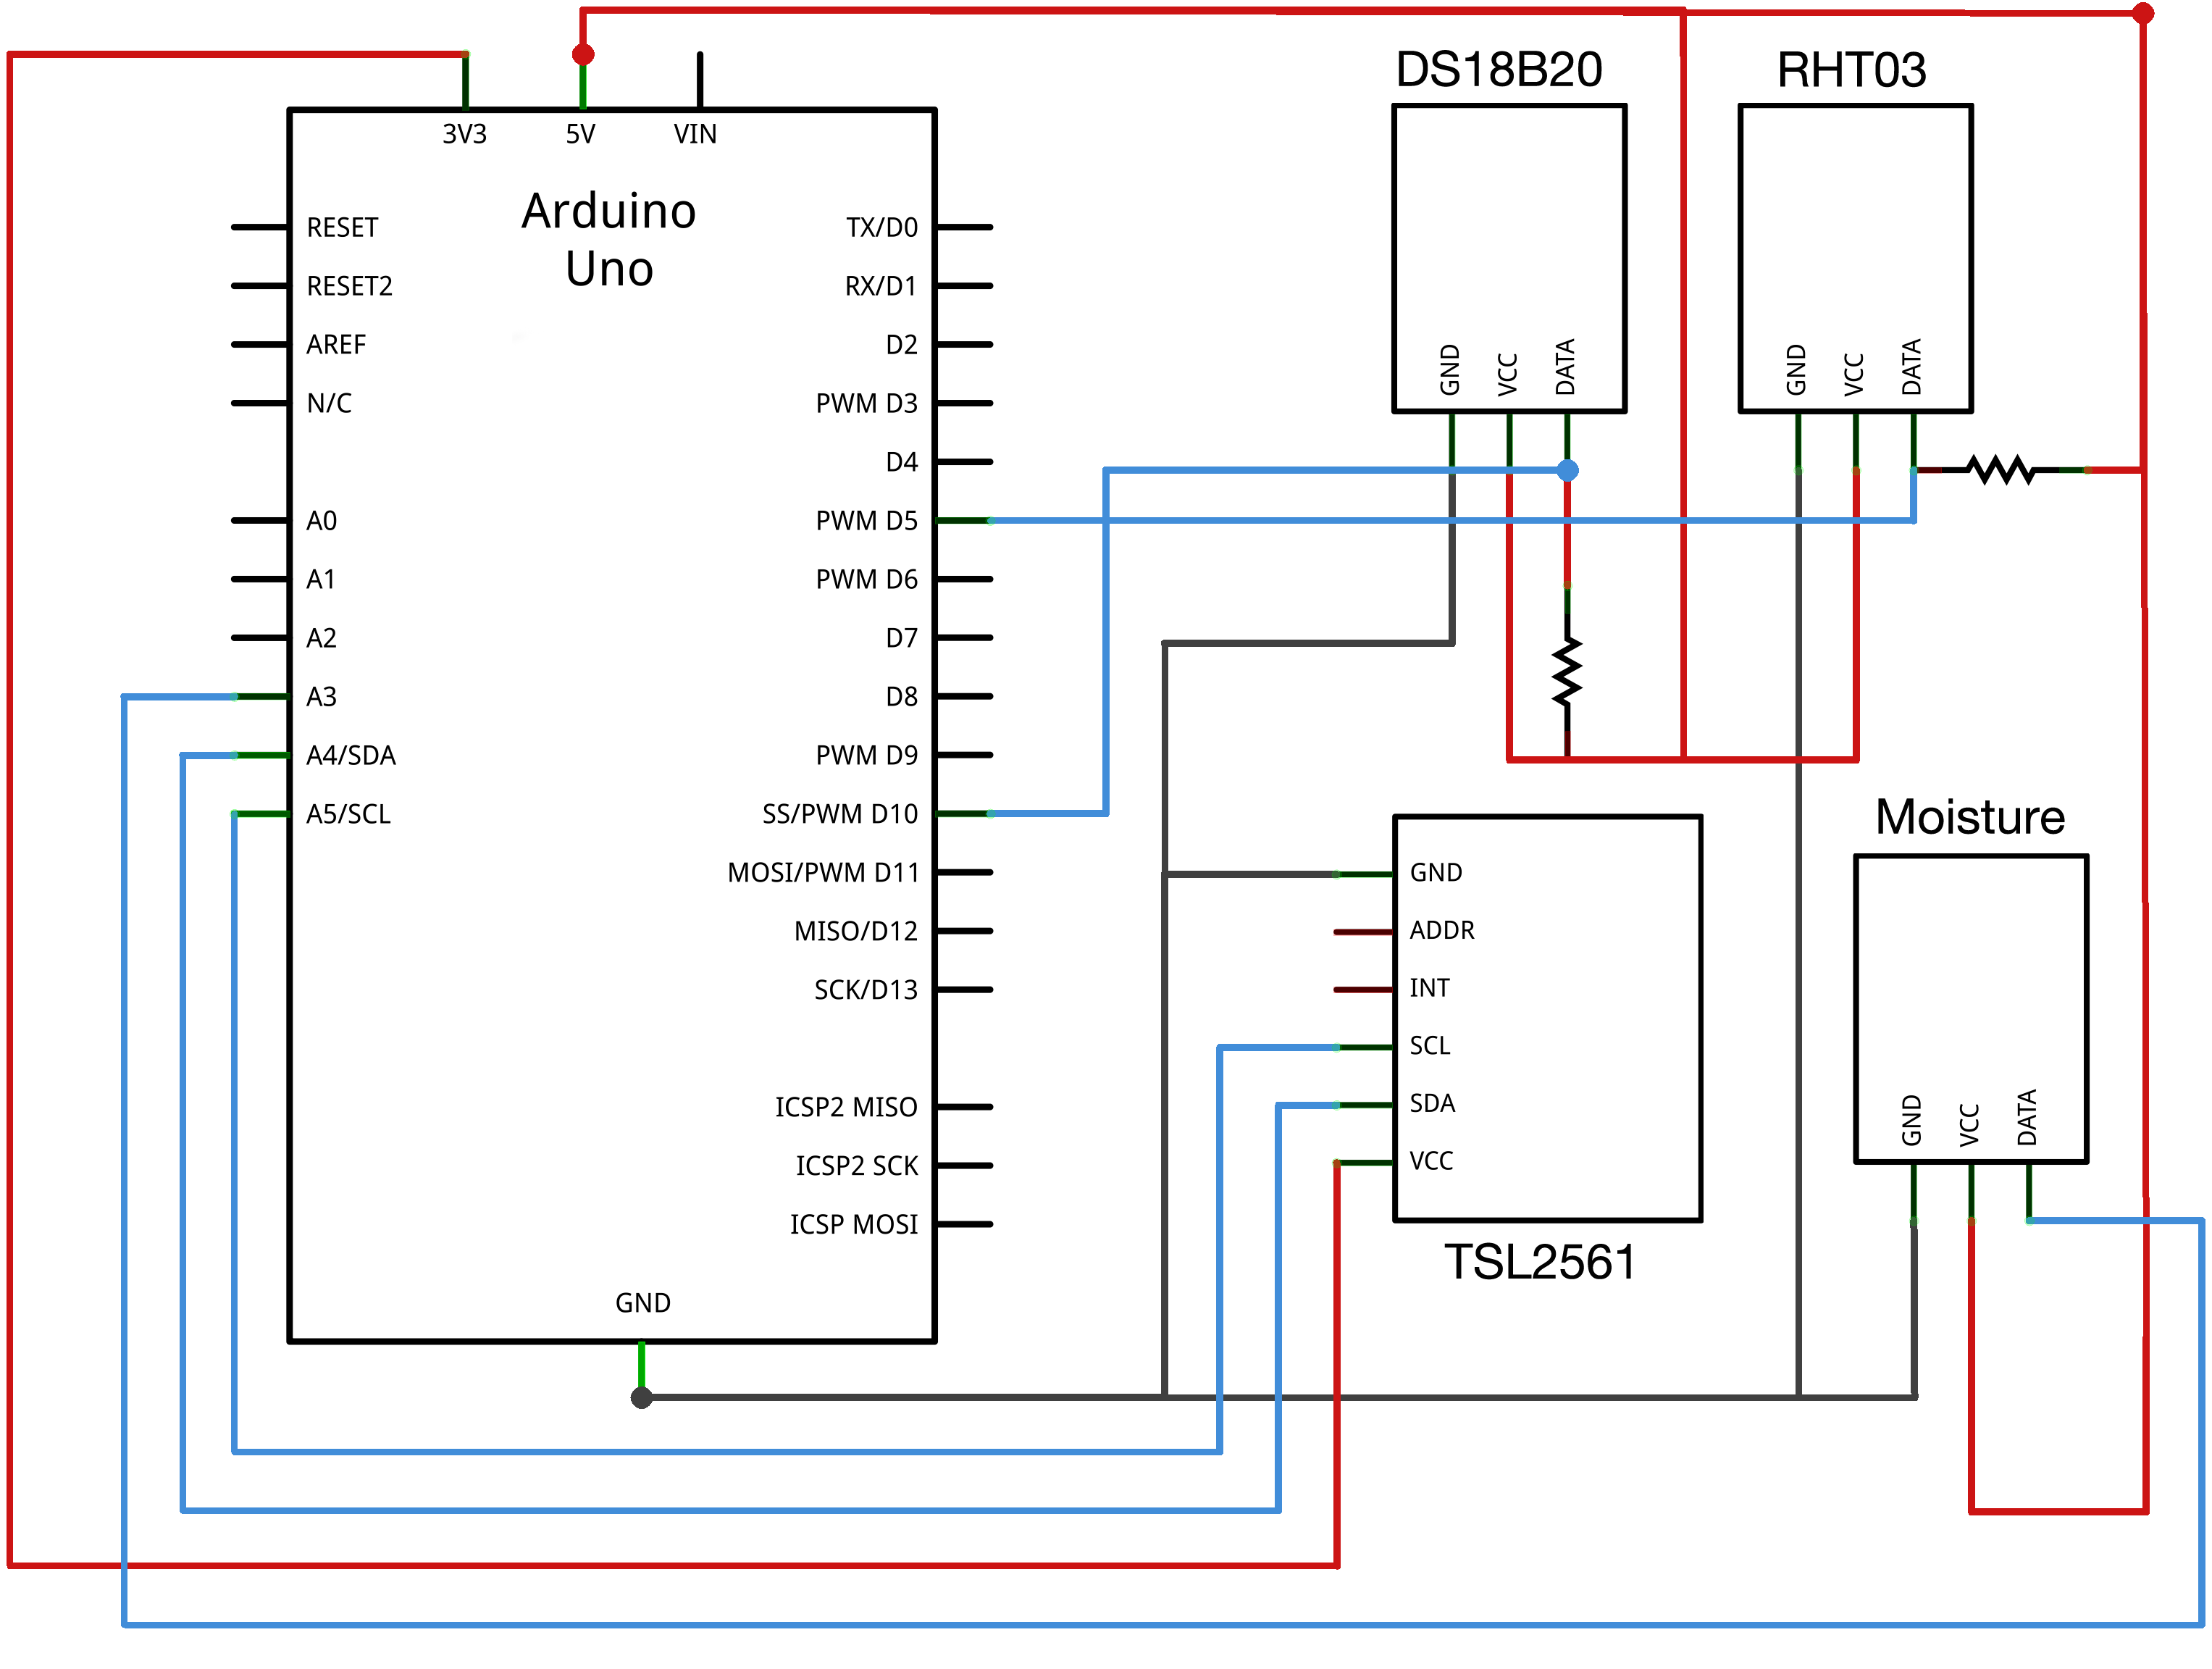
\includegraphics[width=1\textwidth]{img/hardware/Arduino_and_sensors_schem.png}
\caption{Schema diagram of Arduino sensor wiring}
\label{fig:arduino}
\end{figure}

The community surrounding Arduino is quite large, and therefore we were able to find pre-written libraries for communicating with the different sensors. This has made the task of converting the digital signal to the correct units (celsius, relative humidity, lux) and levels a breeze. 

In the case of the soil moisture sensor, it does not output soil moisture in any kind of universal unit. Therefore we measured the resistance in air (high resistance), and in water (low resistance), and let these be the high and low points of a new unit called arbitrary moisture units (AMU).

The code residing in the arduino runs a simple loop where it waits for a special character sent over serial communication through USB. If it receives this character it reads all the sensor values, and sends them back to the next logical unit: the Raspberry Pi

\subsection{Raspberry Pi}
(Why raspberry? Beagleboard?)
The Raspberry Pi is a “cheap, accessible, programmable computer” \citep{raspberrypi} which is roughly the size of a credit card. Our model was released early 2012, and contains two usb ports, audio, sd-card slot, and several GPIO-pins. The devices connected to it are: wireless network adapter, high-definition webcamera, and the Arduino. The operating system running on it is a port of Debian Linux optimized for the Raspberry, called Raspbian. 

(illustration of raspberry)

The GPIO-pins on the raspberry works almost in the same fashion as the Arduino’s digital input output pins. Thus we could in theory simplified the hardware by omitting the Arduino. The main reason for not doing this is that the Raspberry does not have an analog to digital converter (ADC). Therefore we would have to make a complex circuit involving an ADC to interface the Raspberry with the soil moisture sensor. In addition, we would most likely face timing issues. When we ask the digital sensors for data, they send the response immediately. If the unit receiving is not available to read the data, it gets lost. This can be a problem when using a high-level computer, as it performs multiple other tasks in addition to reading sensordata. 

\subsubsection{Operation}
After booting up an endless loop bash-script is called. The script snaps a photo of the plant using the webcam, and then runs a python-script responsible for collecting sensordata. Since we sometimes can get erroneous values from the sensors, we read 15 values and upload the median value.

%http://en.wikibooks.org/wiki/LaTeX/Packages/Listings
\lstset{language=Python} 
\begin{figure}
\begin{lstlisting}
//instantiate lists
airtemp = []
humidity = []
light = []
soiltemp = [] 

for x in xrange(1,15): 
	ser.write("r") //Ask Arduino for data
	variables = ser.readline() //Read the data
	sensorReadings = variables.split('|') //Split string on |

	airtemp.append(float(sensorReadings[0]))
	humidity.append(float(sensorReadings[1]))
	light.append(float(sensorReadings[2]))
	soiltemp.append(float((sensorReadings[3])[:-2])) 

//calculate and post the median using numpy
postData(np.median(airtemp),np.median(humidity),np.median(light),np.median(soiltemp)) 
\end{lstlisting}
\caption{Sensor reading Raspberry Pi}
\label{fig:raspberrycode}
\end{figure}

These values, along with the photo of the plant, are then passed on to the next instance, the API, using pythons HTTP-library urllib2. 

\section{Data processing and database}
When the data has been gathered at the low level hierarchy, it is stored in the cloud. This is done by posting the data to an API on our web server. The main function of an API is to be a mean of communication between software, in our case the data collector and the user interface. After some research on web-API design, we decided that a REST architectual style was the way to go. 

\subsection{Representational State Transfer (REST)}
REST is an architectual style for distributed hypermedia systems \citep{fielding2000architectural}. In Fielding's dissertation, he writes about the interaction constraints of REST that is introduced in order to limit how a distributed system can be constructed. 

\begin{enumerate}
\item{} \emph{Client/Server} - This constraint separates the concerns of the client and the server. By separating these concerns, one secures that the two can evolve independent of each other. The client does not care about the internal logic of the server, and the server doesn't care about what the client does with the data. This gives us the ability to separate the concerns of data collection, data storage and data visualization, which gives us the freedom to change the internal logic of any one of these without worrying about breaking the other two. It also means that we can create several different clients either for collecting data or displaying data.

\item{} \emph{Stateless} - This means that communication between client and server must be stateless. The request from client to server must contain all the information needed to understand the request. In practice this gives the client the responsibility to keep track of the state.

\item{} \emph{Caching} - In order to reduce requests and improve efficiency the server can state which responses can be reused by the client later, when sending equivalent requests. This can greatly enhance user-perceived performance, but at the same time reduce reliability if cached data differs from what would have been delivered by the server on a request. We could theoretically cache almost everything since our data belongs to specific timestamps, and the chances that a sensorvalue is updated at a later time is minimal. However, since we are developing a prototype and have the need for rapid changes in the implementation, we have experienced that the need for reliable data exceeds the need for fast performance.

\item{} \emph{Uniform interface} - This is a rather complex constraint in terms of RESTful API design, and is the reason for a lot of discussions around true REST on various forums on the web. Fielding describes a REST interface to be \emph{“efficient for large-grain hypermedia data transfer, optimizing for the common case of the Web, but resulting in an interface that is not optimal for other forms of architectural interaction.”} \citep{fielding2000architectural} In an applied context this means that the server has resources that can be referenced via URLs and operated through the HTTP-verbs. This means that in order to be a true REST interface, an API can have any resource available through URLs, but the only methods in which one can operate the resource is POST, GET, PUT and DELETE.

\item{} \emph{Layered system} - This constraint tells us that a REST interface may hide complexity in a hierarchical way, by hiding information in such a way that each component cannot "see" beyond the immediate layer with which they are interacting. \citep{fielding2000architectural}

\item{} \emph{Code on demand} - An optional constraint, allowing the server to serve executable code to the client. 

\end{enumerate}

REST is an architectual style, not a strict standard, it allows for flexibility, but at the same time it promotes best practices. The goal of our API was to provide a way of storing and accessing plant data in the cloud, first and foremost for client side applications that we build ourselves. The most important thing was to make something that worked for us. A pragmatic approach to REST gave us the flexibility to create an API that gets the job done. In the following chapter we will describe how the API works and discuss some choices we made in the implementation process.

\subsection{Application Programming Interface - API}
Our first implementation of the API was written in PHP with the framework Codeigniter and a rest-server library as the base. We made a working version, but at some point, after making several dirty workarounds and hacks we started reading about Ruby on Rails and the design paradigm convention over configuration, and soon realized that Rails was exactly what we needed to build our API with.

\begin{quote}
"Ruby on Rails is an open-source web framework that’s optimized for programmer happinees and sustainable productivity. It lets you write beautyful code by favoring convention over configuration."\citep{rubyonrails.org} 
\end{quote}

Ruby on Rails (RoR) is an open-source web framework that makes the assumption that there is a “best” way of doing things, and it encourages that way. It emphasizes well-known software engineering principles such as convention over configuration, don't repeat yourself, model-view-controller and REST.
 Our web server is running on Amazon Elastic Compute Cloud (ec2), a virtual computer service with low costs and extensive configuration options. We chose this because we needed to be able to configure the server for our purposes and install several libraries and applications onto the server. We wanted to create the API The API is created with Ruby on Rails to 

Our API is a server-side Web-API which can be accessed through the HTTP-protocol. This mean that to use it, one can send a request to the domain of the API from any client that has a way to send HTTP-requests. The API will interpret the request and send back a response based on the how the interpretation went. Since our API is based on the REST architectual style, it adheres to how the HTTP-protocol is built, meaning that a resource have a unique identifier a URI, and some uniform actions called the HTTP-verbs which the resource can be operated with. There are 8 methods in the HTTP/1.1 protocol \citep[p.36]{fielding1999hypertext}, but only four of them are of interest when speaking of resources. These methods are the four basic functions of persistent storage in computer programming, often referred to as CRUD (Create, Read, Update and Delete), but in HTTP their names are POST, GET, PUT and DELETE. 

The Monoplant API have three resources: Plants, Sensorvalues and Videos. To create a plant, one can send a POST request to the URL:

\begin{quote}
http://monoplant.me/plants.json 
\end{quote}

A post request also need information about the plant to create, in this case we will pass that information in the json-format:

\begin{figure}
	\begin{lstlisting}[language=javascript]
	 {"plant": {"name": "Alfa", "location": "Intermedia", "plant_type": "Alfalfaspire"}} 
	\end{lstlisting}
	\caption{POST plant json data}
	\label{fig:postdata}
\end{figure}

For the api to know how to interpret this information in json, we also need to pass a parameter in the header called Content-type, this variable will be set to “application/json”. When we pass this request, the API will create a plant with the information we gave it, and give a response with the code: “201 created”. The response contains a header and a body in which the header has some meta-data about the request and the body will contain a representation of the created plant (see figure~\ref{fig:plantresponse} on page~\pageref{fig:plantresponse}).

\begin{figure}
	\begin{lstlisting}[language=javascript]
	{
		created_at: "2013-09-17T10:45:17+02:00"
		id: 1
		location: "Intermedia"
		name: "Alfa"
		plant_type: "Alfalfaspire"
		updated_at: "2013-09-17T10:45:17+02:00"
	}
	\end{lstlisting}
	\caption{Plant response}
	\label{fig:plantresponse}
\end{figure}

If we look at this representation, we see that the API have added an ID to the plant as well as two data attributes created\_at and updated\_at. Since we now have the id of the plant, we can tell the Raspberry Pi to start adding sensor values for the plant. The Raspberry will create a request using the data it gets from the arduino and the image from the web-cam and finally send that POST request to the URL:

\begin{quote}
http://monoplant.me/plants/1/sensorvalues.json 
\end{quote}

As before the API will interpret the request, store the data and respond with a status code: “201 created”. But there is some more stuff happening in the background, the Raspberry only sent the sensorvalues and an image. Internally the API creates a thumbnail of the image and uploads both the thumbnail and the original to another static server, finally storing the URL for both of them in the database. The response body ends up looking like figure~\ref{fig:sensorvaluesresponse}

\begin{figure}
	\begin{lstlisting}[language=javascript]
	{
		airTemp: 22.14
		created_at: "2013-09-17T10:49:43+02:00"
		humidity: 38.5
		id: 10037
		img_url: "http://s3-eu-west-1.amazonaws.com/plantespann/2013/9/17/original/10037.jpg?1379407782"
		light: 1702.5
		photo_content_type: "image/jpeg"
		photo_file_name: "viewcam.jpg"
		photo_file_size: 204358
		photo_updated_at: "2013-09-17T10:49:42+02:00"
		plant_id: 1
		soilMoisture: 54
		soilTemp: 22.25
		thumb_url: "http://s3-eu-west-1.amazonaws.com/plantespann/2013/9/17/thumb/10037.jpg?1379407782"
		updated_at: "2013-09-17T10:49:43+02:00"
	}
	\end{lstlisting}
	\caption{Sensorvalues response}
	\label{fig:sensorvaluesresponse}
\end{figure}

If we need to look at this sensorvalue at a later time, we can simply do a GET request using the sensorvalue id:

\begin{quote}
http://monoplant.me/plants/1/sensorvalues/10037.json 
\end{quote}

This will make the API respond with a status code “302 Found”, and the body will look just like the previous response body, at least if nothing has been updated. Note that the URL is buildt up according to what resource we are trying to operate. See table~\ref{fig:RESTurl} for an overview on how these URLs are built up.

\bgroup
\def\arraystretch{1.8}	%  margin for cells 1 is default
\begin{table}
	\centering
	\begin{tabular}{|c|p{250pt}|} \hline
		\textbf{part of URL}&	\textbf{meaning}\\ \hline
		\texttt{http://}&	the protocol we acces the API through\\ \hline
		\texttt{monoplant.me}&	the domain of the API\\ \hline
		\texttt{/plants/(:id)}&	\texttt{/plants} states that we want to access a resource named plant \\ &
		\texttt{/(:id)} is a number representing the specific plant we want to access\\ \hline
		\texttt{/sensorvalues/(:id)}&	\texttt{/sensorvalues} states that we want to access a resource named sensorvalue, since this comes after \texttt{/plants/(:id)} it means that we will get sensorvalues owned by the plant with \texttt{(:id)}. \\ &
		\texttt{/(:id)} is a number representing the specific sensorvalue we want to operate\\ \hline
		\texttt{(.format)}&	 \texttt{.format} can be blank, .html, .xml or .json. If it is blank, the API will respond with the default format, in our case html. If not it will respond with the corresponding format.\\ \hline
	\end{tabular}
	\caption{How a REST-url is built up}
	\label{fig:RESTurl}
\end{table}
\egroup

\section{User Interface}
The user interface (UI) of monoplant is where we visualize the data from the API to the users. We have built the UI in RoR, HTML, CSS and javascript. The main page represents the current state of the plant, ie. displays the last picture with the corresponding data from the plant. On the right side, there is a time lapse video with a connected graph from the day before (see figure~\ref{fig:mainpage} on page~\pageref{fig:mainpage}).

\begin{figure}
\centering
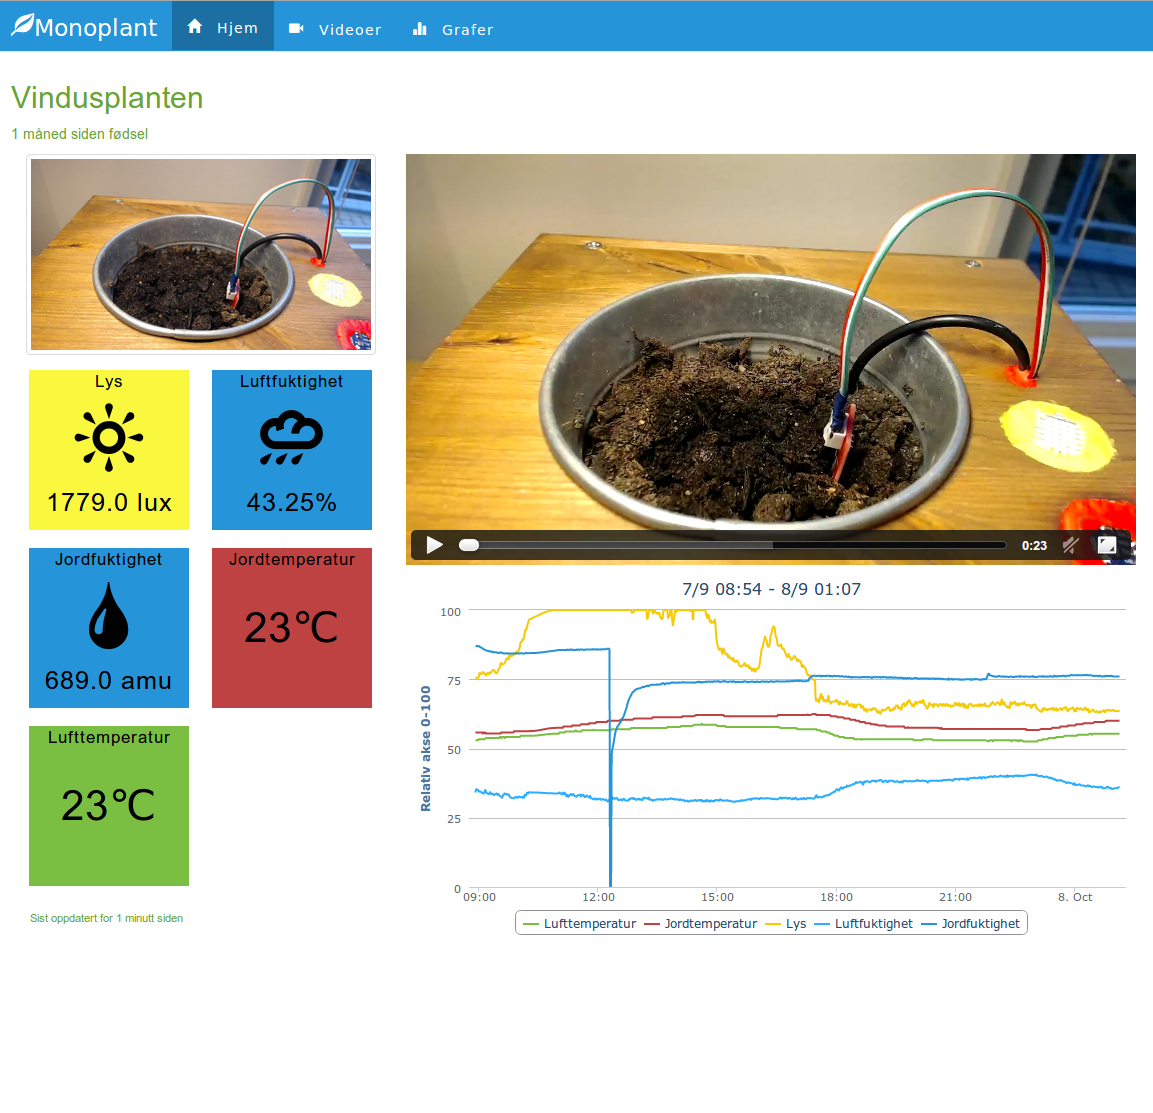
\includegraphics[width=1\textwidth]{img/interface/mainpage.png}
\caption{Screenshot from user interface}
\label{fig:mainpage}
\end{figure}

\subsection{Highcharts}
There are 4-5 serious javascript chart libraries out there with various types of focus, flexibility and documentation. We ran some tests with google charts, d3.js and highcharts, and found that Highcharts provided the most extensive documentation as well as an easy to understand interface, the functionality also made it possible for us to do things we had not thought of earlier.

The first graph we had to make was a graph containing all the plant data from a time corresponding to the timelapse video. This meant putting temperature, light, humidity and soil moisture all in the same graph, even though they all have different units. Out first attempt was done without manipulating the data at all (see figure~\ref{fig:badgraph} on page~\pageref{fig:badgraph}). 

\begin{figure}
\centering
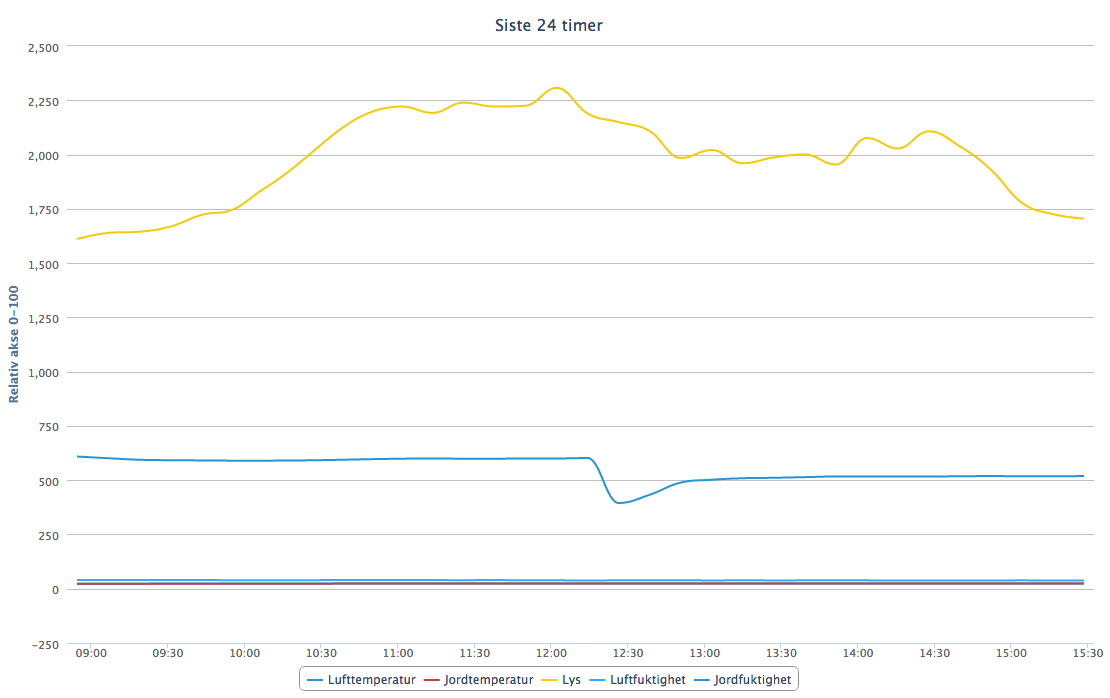
\includegraphics[width=1\textwidth]{img/interface/badgraph.png}
\caption{Screenshot from unsuccessful graph}
\label{fig:badgraph}
\end{figure}

The light data had an average at about 2000 lux, and the temperature was laying at about 22 degrees Celsius. Since highcharts scales the chart based on the data with largest numbers and changes, the data with small numbers and small changes appeared as straight lines at the bottom of the graph. 
For this graph to display the different sensorvalues’ changes over a day, we needed to create a relative scale and map the values to that scale. Lets say you have a number X, which can have a value between A and B, and you want to map it to a value Y between C and D, this becomes a slightly more advanced version of calculating percentage (see figure~\ref{fig:mapfunc} on page~\pageref{fig:mapfunc}).

\begin{figure}
\centering
Y = (X-A)/(B-A) * (D-C) + C
\caption{Map function}
\label{fig:mapfunc}
\end{figure}

We chose an output scale from 0 to 100 and wrote a function according to figure~\ref{fig:mapfunc} that mapped the values based on what type of data it was. We set the input scales as can be seen in figure~\ref{fig:mapscale}.

\begin{figure}
	\begin{lstlisting}[language=javascript]
	humidity: { min: 10, max:100 },
	soil temprature: { min:15, max:30 },
	light: { min: 400, max:2500 },
	air temprature: { min: 15, max: 30 },
	soil Moisture: { min: 0, max: 700 }
	\end{lstlisting}
	\caption{Mapping scales}
	\label{fig:mapscale}
\end{figure}

After running the data through our new function we got a better result and the changes is now visible (see figure~\ref{fig:goodgraph} on page~\pageref{fig:goodgraph}). It will be interesting to see how students interpret this graph, and if they understand that it is a relativ axis. We wanted to keep the information level on this graph down as it will be interpreted alongside the timelapse video and the overhead for interpreting additional information is quite high.  
%Don't know if this should be here, it's not technical, but it's interesting.

\begin{figure}
\centering
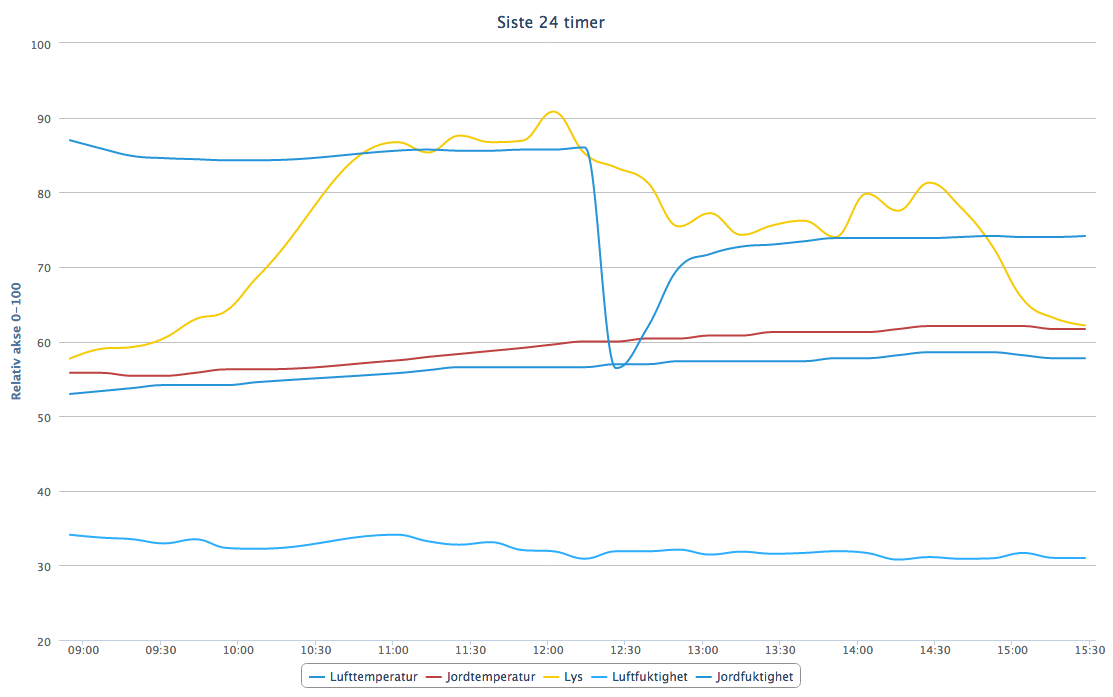
\includegraphics[width=1\textwidth]{img/interface/goodgraph.png}
\caption{Screenshot from succesful graph}
\label{fig:goodgraph}
\end{figure}

To make sure that one can read the appropriate sensorvalues we provide several other graphs, one for the last 24 hours, very similar to the video graph. The only difference is that we have included a mouse-over interaction technique with a tool-tip that displays the actual values alongside with the corresponding image of the plant \citep[p.254]{kluge2010simulation}.

Apart from the video-graph and the last 24 hours-graph we provide singular line graphs for each variable, this gives us the ability to display graphs with correct y-axises. The user can select time period for these graphs by interacting with the small graph on the bottom. 

\subsection{Videoelement}
The html5 specification provides a video-tag for playing videos in the browser, most newer browsers support this, however with varying format-support. Due to the prototypal nature of our application, storage-limits and time constraints we chose to support one video format, and therefore chose h.264 which has the broadest browser support. The video-element can be accessed through javascript, and by checking the state of the video, we are able to make the highcharts graph follow the video based on the currentTime of the videoelement.

\begin{figure}
	\begin{lstlisting}[language=javascript]
	function startVideo(){
	     interval = setInterval(function() {
	         var curtime = video.currentTime.toFixed(2);
	         if(curtime!= lastcurtime){
		 lastcurtime = curtime;
		 curmarker = Math.round(curtime*30);
		 stepTooltip(curmarker);
	         }
	     }, 33);
	}

	function stopVideo(){
		clearInterval(interval);
	}
	\end{lstlisting}
	\caption{Video and graph connection code}
	\label{fig:videocode}
\end{figure}

By binding startVideo() to the play-event of the video-element and stopVideo() to the pause and stop event, we are able to move the graph marker as the video plays. The reason for using setInterval instead of the videos built-in event \emph{timeupdate} is that it is not specified how often the event will fire, but by testing we found that it was somewhere between 3-7 times per second, varying randomly from second to second. This was not often enough as the video had a framerate of 30 frames per second, which meant updating the graph at 1/10 of the speed o the video, resulting in a laggish experience of the graph. We experienced that using setInterval gave use much more accuracy when setting it to run every 33th millisecond. No browsers guarantee that the performance of setInterval will be faster than 50 ms, but by running tests (adequatlygood.com), we found that chrome ran this on an average of 4.5 ms , so we think 33 ms is slow enough for the browser to cope with.
